\documentclass{article}

\usepackage{iclr2026_conference,times}
\input{math_commands.tex}
\usepackage{hyperref}
\usepackage{url}
\usepackage{graphicx}
\usepackage{booktabs}
\usepackage{amsmath}
\usepackage{amssymb}

\title{Contact-Age Invariant Control for Delayed Contact Evidence}

\author{Anonymous Authors}

\newcommand{\lat}{L}
\newcommand{\force}{F}
\newcommand{\qpos}{q}
\newcommand{\qvel}{\dot q}
\newcommand{\ctm}{\Delta}

\begin{document}
\maketitle
\begin{center}
{\small Submission-hardening version: v2 (2026-06-12).}
\end{center}

\begin{abstract}
Contact-rich robot manipulation is usually studied as a problem of force regulation, compliance, planning through contact, or delayed feedback stability. This paper argues for a narrower failure variable: during first contact, delayed tactile or force evidence may describe the wrong \emph{contact age}. A controller can be stable and still accumulate damaging impulse before the delayed contact observation arrives. We study a minimal mechanism, contact-age invariant control, that maintains a contact timing mismatch state, advances delayed contact evidence through a local contact model, and indexes force objectives by inferred contact age rather than wall-clock time or raw delayed force. In a fixed linear Kelvin--Voigt contact mode, the force-advance step exactly cancels constant force-sensing latency when the local stiffness, damping, and proprioceptive state are correct. New ablations narrow the claim: force advancement is the dominant ingredient for latency invariance in this simulator, while contact-age phasing mainly reduces first-contact overshoot. Peak first-contact force for delayed force feedback grows from 9.54 N at zero configured latency to 70.31 N at 150 ms; the full controller remains at 8.48 N in the ideal sweep and has 8.64 N mean peak force at 150 ms over 30 randomized stress seeds. Numeric counterexamples show the claim fails across contact-mode switches and under model mismatch, so the result is a deliberately small but runnable argument for exposing contact timing mismatch as a first-class controller state.
\end{abstract}

\section{Introduction}

Robots that manipulate through contact must react to events that are both mechanical and semantic. The instant a gripper, tool, or end-effector touches the world, the control problem changes: position error becomes penetration, velocity becomes impact, and a force sample becomes meaningful only if its timestamp belongs to the current contact mode. This is uncomfortable for controllers that treat sensing latency as ordinary delayed feedback. A delayed force sample is not merely old; at first touch it may be evidence from the wrong side of a hybrid guard.

The research bet in this paper is that \emph{contact timing mismatch} should be a controller state. Let the physical contact age be the time since the contact event actually occurred, and let the observation age be the time since the controller's delayed evidence indicates contact. The difference between these quantities, denoted $\ctm$, is the hidden variable that explains why an otherwise stable force controller can push too hard during the blind interval after first touch.

We propose a minimal contact-age invariant controller. It has three parts: estimate or infer the contact event time; advance stale force evidence through a local contact model using current proprioception; and phase the desired force ramp by inferred contact age. This is not claimed as a new impedance controller, a new Smith predictor, a passivity theorem, reinforcement learning, or a benchmark. Its purpose is to isolate a mechanism that prior clusters often leave implicit: the controller state must encode the mismatch between when contact physically began and when contact evidence says it began.

The contribution is intentionally scoped.
\begin{itemize}
    \item We identify a field assumption: delayed contact evidence remains semantically aligned with the current contact mode.
    \item We give a small algebraic claim: in a known linear contact mode, delayed force can be advanced exactly using current-minus-delayed proprioception.
    \item We provide runnable evidence in a one-dimensional contact task, including ablations that separate force advancement from contact-age target phasing and a 30-seed randomized stress test.
    \item We mark the strongest limitations: no hardware, no global contact-mode proof, no claim under arbitrary frictional contact, and only abstract-level automated literature coverage beyond the closest cited works.
\end{itemize}

\section{Related Work And Hostile Prior Art}

\paragraph{Force, impedance, and hybrid contact control.}
Classical force and compliance control already establish much of the surface area of this problem. Hybrid position/force control separates constrained and unconstrained directions \citep{raibert1981hybrid}, compliance and force control regulate interaction with constrained environments \citep{mason1981compliance}, and impedance control shapes the apparent endpoint dynamics \citep{hogan1985impedance}. Cooperative and multi-arm variants extend these ideas to object-level impedance and constrained manipulation \citep{schneider1992object,yoshikawa1993coordinated}. Modern contact-rich manipulation and force-control learning papers show that force regulation remains central in data-driven systems \citep{beltran2020learning,suomalainen2022survey}. These works make compliant force regulation non-novel. Our boundary is narrower: the force objective should be indexed by inferred contact age when contact evidence is delayed.

\paragraph{Delay, passivity, and teleoperation.}
Time-delay control and teleoperation have a mature literature. Smith predictors compensate known dead time in continuous processes \citep{smith1957closer}. Bilateral teleoperation under communication delay uses passivity, scattering, or layered passivity/transparency methods to avoid unstable energy injection \citep{anderson1989bilateral,niemeyer1991stable,stramigioli2005sampled,franken2011bilateral}. These works are the closest hostile cluster because they make generic delay compensation and stable delayed force channels non-novel. The distinction is that first contact is a hybrid semantic event. A stable delayed channel can still report a pre-contact force sample while the robot is already accumulating contact impulse.

\paragraph{Planning and learning through contact.}
Trajectory optimization through rigid contact \citep{posa2013direct} and contact-rich policy learning \citep{levine2015learning} model or learn the mechanics of intermittent contact. They make the idea of using a contact model non-novel. The present work does not add a bigger model or a reinforcement learner. It asks what state variable the controller should expose when contact observation latency changes without changing geometry or dynamics.

\paragraph{Recent force and tactile policies.}
Recent manipulation systems increasingly add force or tactile streams to learned policies, data collection, or predictive tactile models. Examples include force-conditioned grasp-policy data \citep{xie2024just}, slow-fast visual-tactile policy learning with high-frequency tactile feedback \citep{xue2025reactive}, and force-guided tactile foresight for contact-rich manipulation \citep{zang2026tacforesight}. These papers are hostile to any broad claim that force/tactile feedback for contact-rich manipulation is new. Our boundary is narrower and more classical: before learning a rich policy, a controller may need to represent whether the force/tactile evidence belongs to the current contact age.

\section{Problem Setup}

Consider a one-dimensional robot endpoint with position $\qpos_t$, velocity $\qvel_t$, and unilateral contact at $\qpos_t > 0$. In contact, force follows a local Kelvin--Voigt model
\begin{equation}
    \force_t = k \qpos_t + c \qvel_t,
    \quad \qpos_t > 0,
\end{equation}
with stiffness $k$ and damping $c$. Force or tactile evidence is observed after latency $\lat$, while proprioceptive position and velocity are assumed timestamped and effectively current at the control rate. This assumption is strong, but common on real robots where joint encoders are much faster and closer to the servo loop than tactile image processing or external force perception.

The controller's hidden timing variable is
\begin{equation}
    \ctm_t = (t - \hat t_c) - (t - \lat - \hat t_c^{obs}),
\end{equation}
where $\hat t_c$ is the inferred physical contact time and $\hat t_c^{obs}$ is the contact time implied by delayed evidence. In the simple simulator, $\hat t_c$ is detected from the known contact guard. In less ideal systems it could be estimated from expected geometry, proprioceptive residuals, or a delayed force edge corrected by an online latency estimate. This paper studies the local mechanism, not a full estimator.

\section{Contact-Age Invariant Control}

At time $t$, the controller receives delayed force $\force_{t-\lat}$ and delayed proprioceptive state $(\qpos_{t-\lat},\qvel_{t-\lat})$, but also has current proprioception $(\qpos_t,\qvel_t)$. If both samples are in the same linear contact mode, the current force is reconstructed by
\begin{equation}
    \hat \force_t =
    \force_{t-\lat}
    + \hat k(\qpos_t-\qpos_{t-\lat})
    + \hat c(\qvel_t-\qvel_{t-\lat}).
    \label{eq:advance}
\end{equation}
When the delayed sample is pre-contact but current proprioception indicates contact, the controller advances from the inferred contact event rather than waiting for the delayed force edge:
\begin{equation}
    \hat \force_t = \max(0, \hat k \qpos_t + \hat c \qvel_t).
\end{equation}
The target force is phased by contact age $\tau_c = t-\hat t_c$:
\begin{equation}
    \force_t^\star = \min(\force_{\max}, r \tau_c),
\end{equation}
where $r$ is a force ramp rate. The commanded velocity is a clipped proportional force action,
\begin{equation}
    u_t = \mathrm{clip}\left(g(\force_t^\star - \hat \force_t), -u_{\max}, u_{\max}\right).
\end{equation}
The key difference from delayed-force feedback is not the proportional law; it is the state used to evaluate the law. Delayed feedback compares the current objective to stale force. Contact-age control compares a contact-age objective to an advanced estimate of current force.

\paragraph{Formal claim and boundary.}
If $\hat k=k$, $\hat c=c$, both delayed and current samples are in the same unclipped Kelvin--Voigt contact mode, and proprioception is exact, then Eq.~\ref{eq:advance} gives $\hat \force_t=\force_t$ for any constant latency $\lat$. The proof is substitution:
\begin{align}
\hat \force_t
&= (k\qpos_{t-\lat}+c\qvel_{t-\lat})
 + k(\qpos_t-\qpos_{t-\lat})
 + c(\qvel_t-\qvel_{t-\lat}) \\
&= k\qpos_t+c\qvel_t
 = \force_t .
\end{align}
This is the whole formal guarantee. It is not a global hybrid-system theorem. Our claim checker verifies the same-mode residual to floating-point tolerance and finds counterexamples when a delayed pre-contact sample is naively advanced across a mode switch.

\section{Experiments}

\paragraph{Simulator.}
We use a minimal point endpoint approaching a rigid contact. The plant receives velocity commands through a first-order servo, contact force is Kelvin--Voigt, and the task is to reach an 8 N contact force. We sweep force/tactile sensing latency from 0 to 150 ms. Five controllers are compared: delayed force feedback; a delay-scaled cautious baseline that slows the blind approach as latency grows; force advancement without contact-age target phasing; contact-age target phasing without force advancement; and the full controller. All scripts are in the repository: \texttt{scripts/run\_experiments.py} produces the CSV, JSON, and figures; \texttt{scripts/verify\_claims.py} produces the formal audit and counterexamples.

\begin{figure}[t]
    \centering
    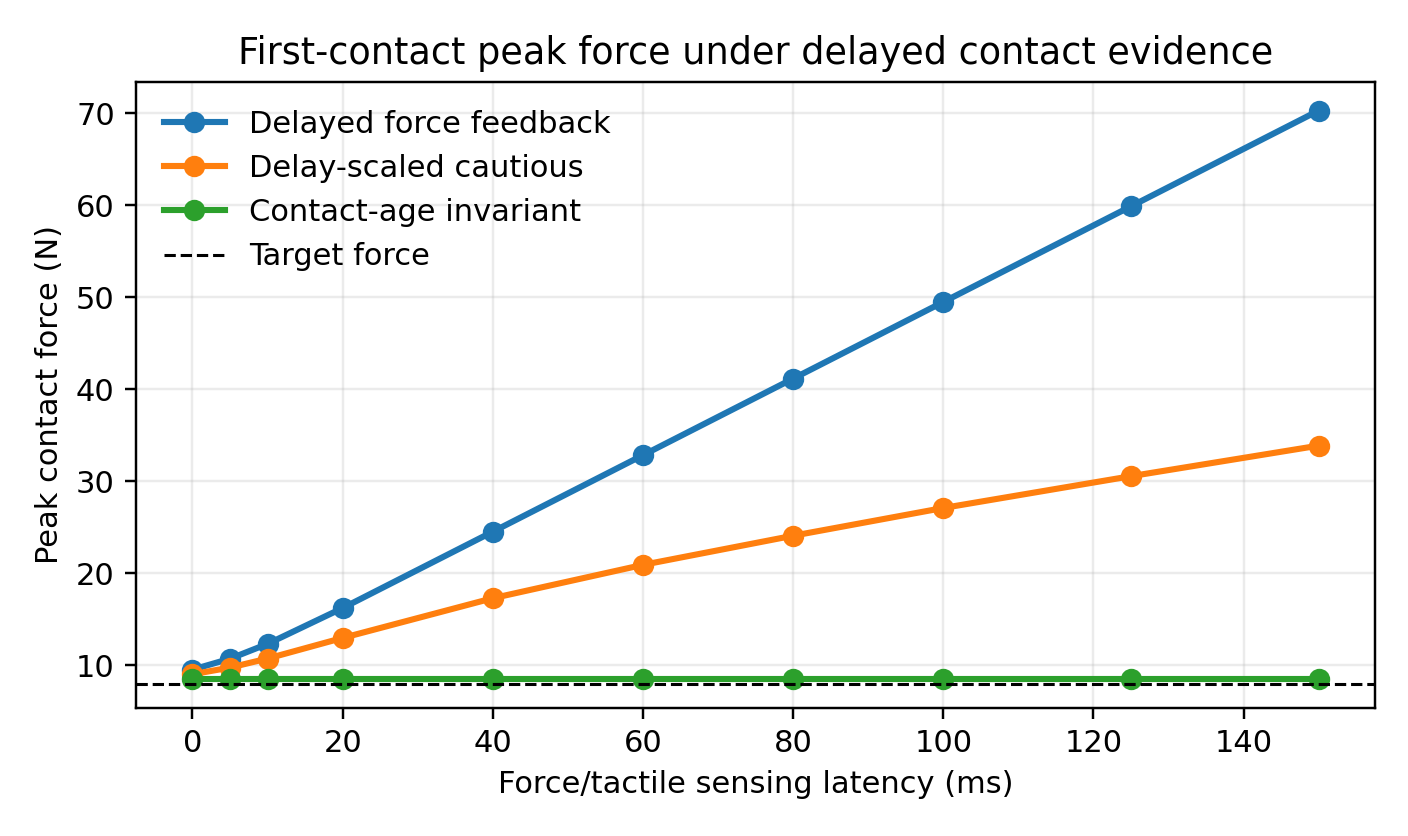
\includegraphics[width=0.86\linewidth]{figures/peak_force_vs_latency.png}
    \caption{Peak first-contact force as force/tactile sensing latency increases. Delayed feedback accumulates contact impulse before the force edge arrives. The contact-age controller remains nearly latency invariant in this local model because it advances delayed force evidence and phases the target by inferred contact age.}
    \label{fig:peak}
\end{figure}

\begin{table}[t]
    \centering
    \caption{Latency sweep summary. Slopes are peak-force change per second of sensing latency. Lower peak and lower slope are better.}
    \label{tab:summary}
    \begin{tabular}{lccc}
        \toprule
        Controller & Max peak (N) & Mean overshoot (N) & Peak slope (N/s) \\
        \midrule
        Delayed force feedback & 70.31 & 24.71 & 410.13 \\
        Delay-scaled cautious & 33.89 & 11.64 & 169.74 \\
        Force advancement only & 9.04 & 1.04 & 0.00 \\
        Contact-age target only & 70.32 & 23.74 & 427.59 \\
        Contact-age invariant & 8.48 & 0.48 & $<10^{-12}$ \\
        \bottomrule
    \end{tabular}
\end{table}

Figure~\ref{fig:peak} and Table~\ref{tab:summary} show the main result. The delayed controller is acceptable near zero latency but becomes unsafe as the blind interval grows. The cautious controller reduces the slope but still lets peak force rise with latency and sacrifices final regulation at larger delays. The contact-age controller's peak force is constant in the ideal local model because the controller's force estimate is no longer indexed by delayed observation time.

\begin{figure}[t]
    \centering
    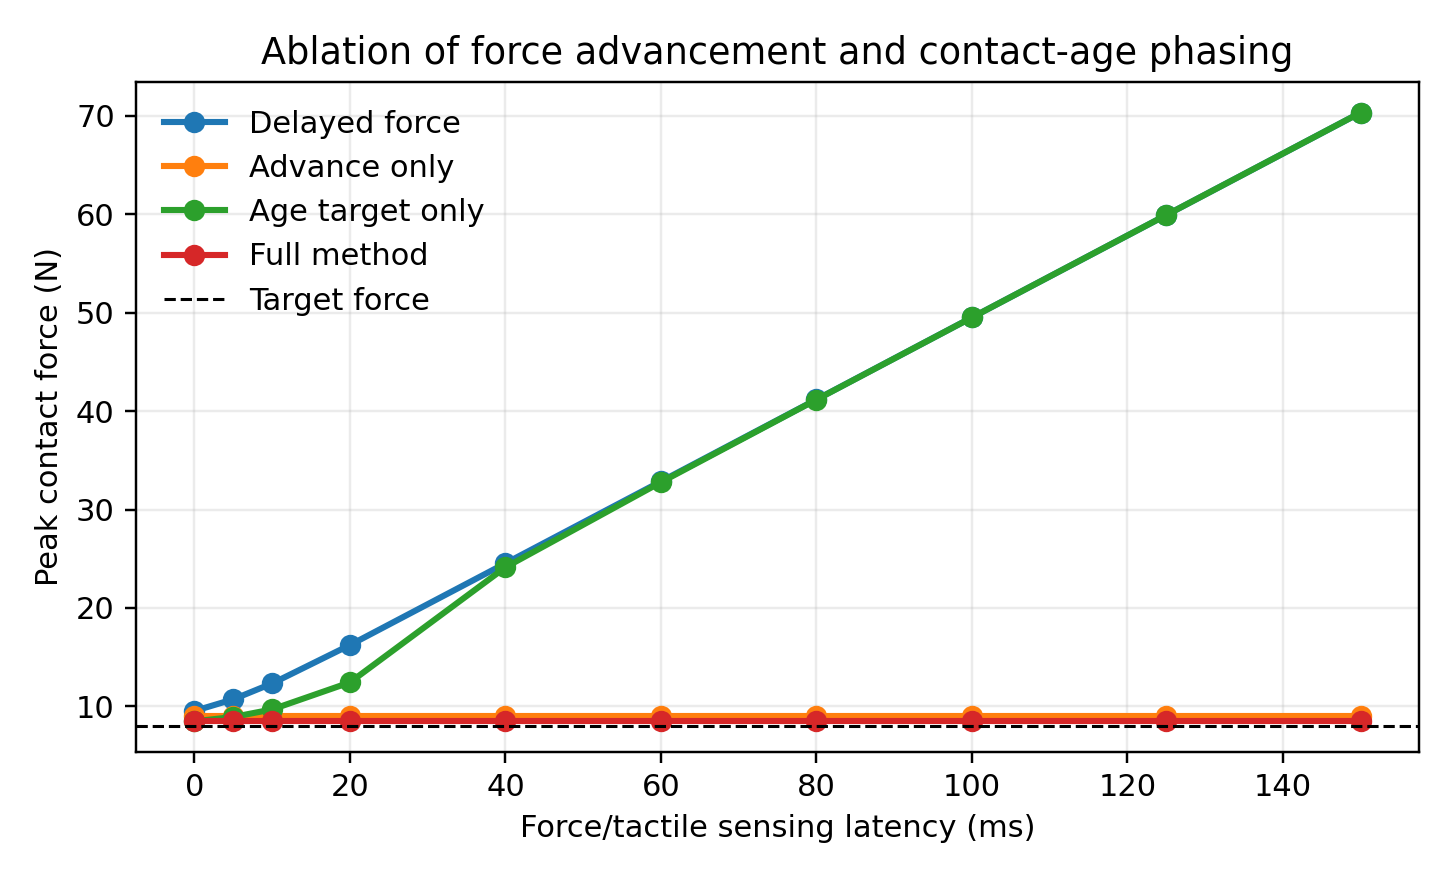
\includegraphics[width=0.86\linewidth]{figures/mechanism_ablation.png}
    \caption{Mechanism ablation. Force advancement alone removes most latency sensitivity in this local simulator, while contact-age target phasing alone does not. The full controller gives the lowest first-contact peak but the ablation narrows the novelty claim: event-age phasing is a safety shaping layer on top of local force advancement, not the sole source of invariance.}
    \label{fig:ablation}
\end{figure}

Figure~\ref{fig:ablation} is deliberately adversarial. It shows that force advancement is the dominant ingredient for latency invariance in the one-dimensional model. Contact-age target phasing alone tracks the delayed-force failure mode because it still compares the target against stale force evidence. The full method improves the peak from 9.04 N to 8.48 N relative to force advancement alone, but this is a modest overshoot improvement, not a separate proof of novelty over prediction-based delay compensation.

\begin{figure}[t]
    \centering
    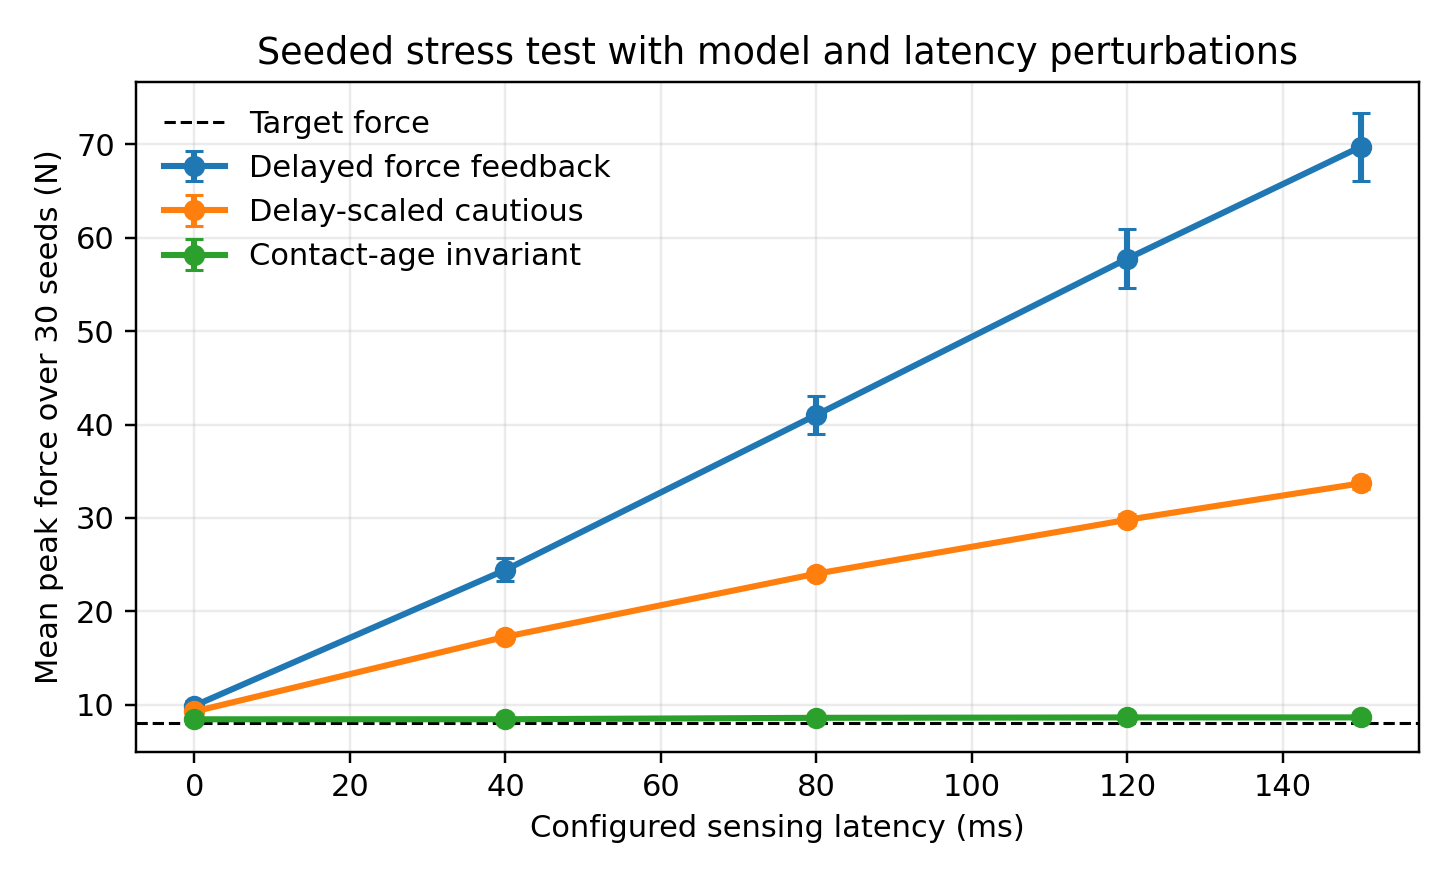
\includegraphics[width=0.86\linewidth]{figures/seeded_stress_peak_force.png}
    \caption{Seeded stress test over 30 random seeds with stiffness, damping, servo time constant, initial gap, model-estimate, and effective-latency perturbations. Markers show mean peak force; error bars are 95 percent confidence intervals over seeds.}
    \label{fig:stress}
\end{figure}

We also run a 30-seed stress test with randomized stiffness, damping, servo time constant, initial gap, stiffness/damping estimates, and effective latency. At 150 ms configured latency, delayed force feedback reaches $69.75\pm3.66$ N mean peak force, the delay-scaled cautious baseline reaches $33.71\pm0.60$ N, and the full controller reaches $8.64\pm0.40$ N. Across all stress runs, the full controller exceeds 12 N in 1.3 percent of runs, compared with 80.7 percent for both delayed force feedback and the cautious baseline. The stress test therefore supports bounded robustness in this local model, not deployment readiness.

\paragraph{Adversarial checks.}
The formal audit reports a same-mode maximum residual of $7.1\times10^{-15}$ N for 10,000 random samples. It also finds a mode-switch counterexample with 25.93 N residual for a naive force-advance rule applied across pre-contact to post-contact samples. With a 15 percent stiffness error and 15 percent damping error in opposite directions, the mean force-prediction residual is 1.28 N and the max residual is 3.86 N. These failures are important: exact invariance requires the local model and contact mode to be right. The ablation in Figure~\ref{fig:ablation} adds another boundary: this paper must not claim that contact-age phasing alone solves delayed contact evidence.

\section{Limitations}

This is not a hardware paper. The evidence is a controlled one-dimensional simulator designed to isolate a timing assumption. The method assumes fast timestamped proprioception and a useful local contact model. Unknown geometry, deformable contact, stick-slip friction, actuator saturation, and unobserved contact modes can break the mechanism. The new ablation weakens the original rhetorical position: in this simulator, force advancement alone is already nearly latency invariant, so the contribution cannot be sold as a wholly new alternative to prediction-based delay compensation. The honest claim is that representing contact event age exposes when local prediction is semantically valid, when it crosses a hybrid boundary, and how force targets should be phased at first contact. The literature sweep contains 1242 OpenAlex entries and a 100-paper hostile set, but the automated 225-paper deep tier is an abstract/metadata classification rather than a manual full-PDF read. The correct readiness judgment is therefore conservative: the idea is plausible and runnable, but it needs multi-DOF simulation, tactile timestamp estimation, and hardware validation before a strong conference submission.

\section{Conclusion}

Contact latency in manipulation is not only a delayed signal problem. At first contact, it is a delayed hybrid-event semantics problem. Treating the contact timing mismatch as a state variable leads to a simple controller that advances delayed force evidence and phases force objectives by contact age. In the local linear-contact regime this cancels constant force-sensing latency exactly; outside that regime, the same formal check exposes the failure modes. The ablation clarifies the mechanism: local force advancement carries most of the invariance, and contact-age phasing reduces first-contact overshoot. The broader lesson is that embodied controllers should sometimes be invariant to observation time by moving into event-age coordinates, but this paper is only a local simulation argument for that design principle.

\bibliography{references}
\bibliographystyle{iclr2026_conference}

\end{document}
